\chapter{Comparison}
%
% 3.1
{ \textbf{3.1 {YOLO vs Traditional and Deep-Learning Object Detection Methods}}}\newline
\newline
%
Object detection has evolved from traditional methods like HOG+SVM and Haar Cascades to advanced deep learning models such as YOLO, Faster R-CNN, and EfficientDet. Traditional approaches struggle in complex environments, while deep learning models provide superior speed and accuracy. Among them, YOLO stands out for its real-time performance, making it ideal for applications like autonomous driving and surveillance, where speed is critical.\\\\
%
%
  \begin{figure}[h!]
    \centering
    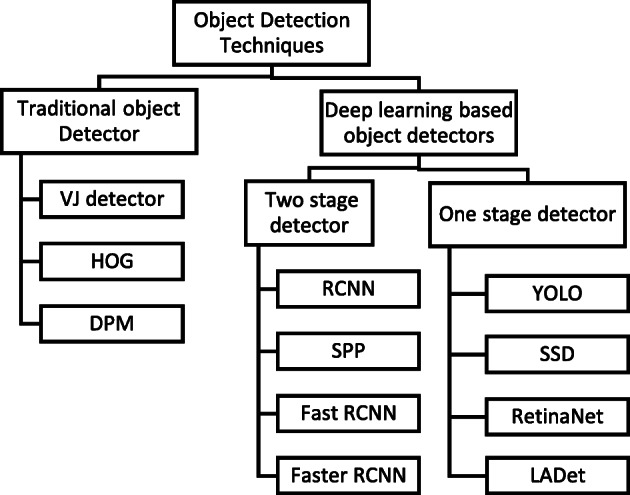
\includegraphics[width=0.5\textwidth]{images/Object Detection Techniques.png}
    \caption{Object Detection Techniques}
    \label{fig:enter-label}
  \end{figure}
\\\\\\
%
%
YOLO surpasses traditional methods like HOG+SVM and Haar Cascades in every aspect. Traditional methods rely on hand-engineered features, which are less robust in complex environments. YOLO’s ability to learn features directly from data makes it much more adaptable and accurate in real-world scenarios. Traditional methods also lack the capability to process multiple objects efficiently and are unsuitable for tasks requiring real-time detection, unlike YOLO, which excels in these areas.\\
%
% Table 1
\begin{table}[ht]
\centering
\caption{YOLO vs Traditional Methods}
\vspace{0.3cm} 
\begin{tabular}{|l|l|l|p{4.5cm}|p{4.5cm}|}
\hline
\textbf{Method}       & \textbf{Speed} & \textbf{Accuracy} & \textbf{Strengths}                                 & \textbf{Weaknesses}                               \\ \hline
\textbf{YOLO}         & 30-45 FPS      & High             & Learns features automatically, real-time capable  & Struggles with small objects                     \\ \hline
\textbf{HOG+SVM}      & Slow           & Low              & Simplicity, low computational cost                & Fails in complex environments                    \\ \hline
\textbf{Haar Cascades} & Moderate       & Low              & Efficient for simple tasks                        & Limited object variety, low accuracy             \\ \hline
\end{tabular}
\label{tab:yolo_vs_traditional}
\end{table}
\\\\
%
%
While methods like Faster R-CNN, RetinaNet, and EfficientDet offer higher accuracy, YOLO remains the leading choice for real-time object detection due to its exceptional speed. YOLO processes the entire image in a single forward pass, eliminating the need for region proposals or multi-scale feature extraction, which slows down other methods. This efficiency, combined with a strong balance between speed and accuracy, makes YOLO the preferred method for applications like autonomous driving, surveillance, and robotics, where every millisecond counts. combine this with above one.
%
% Table 2
\begin{table}[H]
\centering
\caption{Comparison of YOLO with Other Deep Learning Methods}
\vspace{0.3cm} 
\begin{tabular}{|l|c|c|p{3.5cm}|p{3.5cm}|}
\hline
\textbf{Method}       & \textbf{Speed}         & \textbf{Accuracy} & \textbf{Strengths}                       & \textbf{Weaknesses}                          \\ \hline
\textbf{YOLO}         & 30-45 FPS              & High              & Real-time detection                      & Struggles with small objects                 \\ \hline
\textbf{Faster R-CNN} & Moderate (10 FPS)      & Very High         & High accuracy, good for complex scenes   & Slower than YOLO due to region proposals     \\ \hline
\textbf{RetinaNet}    & Moderate (5-15 FPS)    & High              & Focuses on dense object detection        & More complex architecture, slower inference  \\ \hline
\textbf{EfficientDet} & Moderate               & Very High         & Efficient scaling, high accuracy         & Requires more computational resources        \\ \hline
\textbf{SSD}          & 20-40 FPS              & High              & Fast detection, suitable for real-time applications & Struggles with detecting smaller objects     \\ \hline
\textbf{Mask R-CNN}   & Slow (5-10 FPS)        & Very High         & Can detect objects and generate segmentation masks & Slower due to additional segmentation steps  \\ \hline
\textbf{Cascade R-CNN}& Slow (5-10 FPS)        & Very High         & High accuracy, especially for detecting objects at different scales & Computationally expensive, slow inference    \\ \hline
\end{tabular}
\label{tab:yolo_vs_other_methods}
\end{table}
%
% 
\begin{figure}[H]
    \centering
    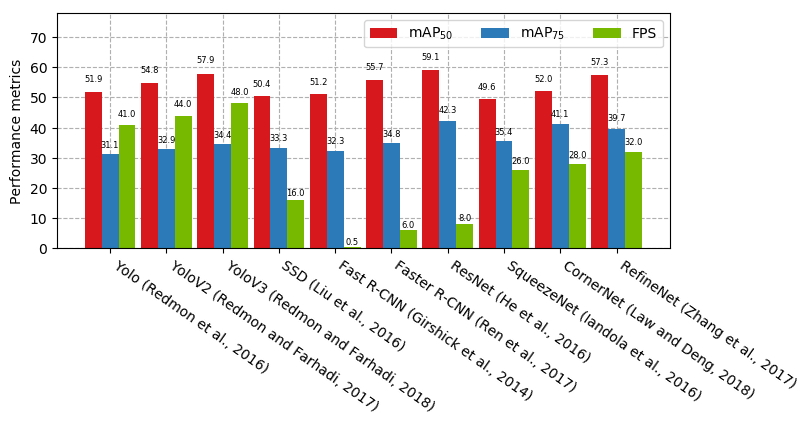
\includegraphics[width=0.9\textwidth]{images/Yolo vs Other Models.png}
    \caption{Performance Metrics of Object Detection Techniques on Pascal VOC 2012 Dataset}
    \label{fig:performance_metrics}
\end{figure}
%
% Section 3.2
\section*{3.2 YOLOv1 - YOLOv8}
The YOLO (You Only Look Once) object detection algorithm, introduced by Joseph Redmon in 2016, revolutionized object detection by offering a real-time approach with high accuracy and speed. Unlike traditional methods, YOLO treats object detection as a single regression problem, predicting bounding boxes and class probabilities from full images. Over the years, YOLO has undergone significant evolution. YOLOv1 pioneered real-time detection but struggled with small objects. YOLOv2 introduced anchor boxes and batch normalization for better accuracy, while YOLOv3 improved detection using a deeper network and multi-scale predictions. YOLOv4 introduced advanced techniques like PANet and self-adversarial training, further boosting performance. YOLOv5 gained popularity for its ease of use and mobile optimization, while YOLOv6 and YOLOv7 further refined speed and accuracy. YOLOv8, the latest version, offers the most advanced architecture, excelling in both speed and accuracy across multiple tasks. Each version allows customization and fine-tuning for specific applications, making YOLO highly versatile in various object detection tasks.
%
%
  \begin{figure}[h!]
    \centering
    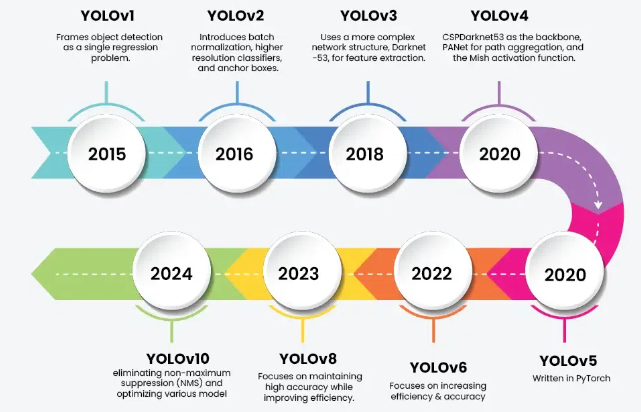
\includegraphics[width=0.5\textwidth]{images/Yolo Timeline.png}
    \caption{YOLO Timeline}
    \label{fig:enter-label}
  \end{figure}\\
%
%
YOLO versions can be easily modified and customized for specific tasks through transfer learning and fine-tuning on custom datasets. Users can adjust anchor box dimensions, change the number of output classes, or alter the architecture by adding or removing layers, depending on the use case. Additionally, modifications can include changes to the architecture (CA) and loss functions to enhance performance (Eg: YOLOv8-CAW model). The introduction of algorithms designed to overcome specific drawbacks found in previous variants further improves their efficacy (Eg: Outlier Rejection and Linear Interpolation). The simplicity of the YOLO architecture also allows for seamless integration with other algorithms (e.g., attention mechanisms, R-CNN features) for enhanced performance. 
%
% Table 3
\begin{table}[ht]
\centering
\caption{Comparison of YOLO Versions}
\vspace{5pt} 
\begin{tabular}{|p{1.8cm}|p{1.2cm}|p{2.5cm}|p{1.8cm}|p{1.8cm}|p{5.5cm}|} 
\hline
\textbf{Version} & \textbf{Year} & \textbf{Backbone} & \textbf{Speed (FPS)} & \textbf{Accuracy \small{(mAP@50)}} & \textbf{Key Features} \\ \hline
YOLOv1  & 2016 & Custom CNN       & 45 FPS   & 63.4\%  & Single-scale detection, simple architecture \\ \hline
YOLOv2  & 2017 & Darknet-19       & 67 FPS   & 76.8\%  & Anchor boxes, batch normalization, multi-scale detection \\ \hline
YOLOv3  & 2018 & Darknet-53       & 30 FPS   & 78.6\%  & Residual blocks, multi-scale predictions, feature pyramids \\ \hline
YOLOv4  & 2020 & CSPDarknet53     & 60 FPS   & 89.7\%  & PANet, SAT, advanced data augmentation, efficient backbone \\ \hline
YOLOv5  & 2020 & Focus + CSPNet   & 140 FPS  & 88.0\%  & PyTorch implementation, easy deployment, mobile-friendly \\ \hline
YOLOv6  & 2022 & EfficientRep     & 150+ FPS & 89.6\%  & EfficientRep backbone, optimized for GPUs, better quantization \\ \hline
YOLOv7  & 2022 & E-ELAN           & 160 FPS  & 90.2\%  & Model re-parameterization, versatile architecture \\ \hline
YOLOv8  & 2023 & Ultralytics Backbone & 170 FPS  & 91.0\%  & Advanced architecture, improved support for multiple tasks \\ \hline
\end{tabular}
\label{tab:yolo_versions}
\end{table}
%
%
  \begin{figure}[h!]
    \centering
    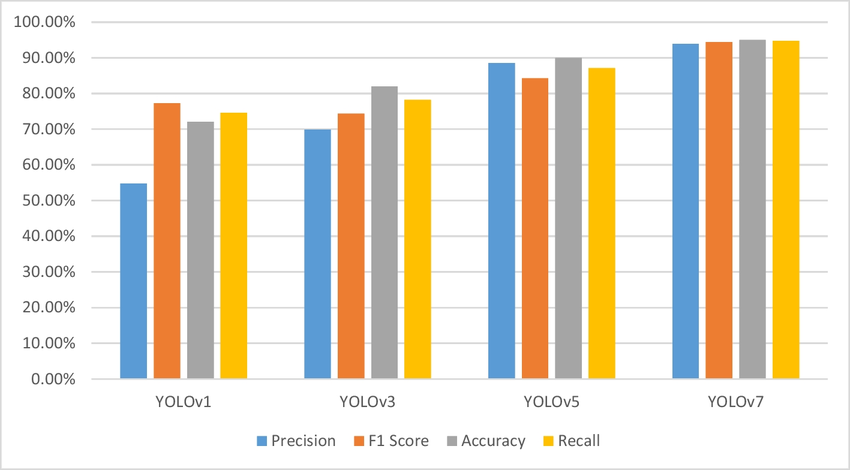
\includegraphics[width=0.7\textwidth]{images/Yolo Variants Performance Metrics.png}
    \caption{YOLO Variants Performance Metrics}
    \label{fig:enter-label}
  \end{figure}
%
%